%%%%%%%%%%%%%%%%%%%%%%%%%%%%%%%%%%%%%%%%%%%%%%%%%%%%%%%%%%%%%%%%%%%%%%%%%%%%%%%%
%% Title (en): Multiagent Systems and Organizations                           %%
%% Title (cs): Multiagentní systémy a organizace                              %%
%%                                                                            %%
%% Author: Bc. Lukáš Kúdela                                                   %%
%% Supervisor: Prof. RNDr. Petr Štěpánek, DrSc.                               %%
%%                                                                            %%
%% Academic year: 2011/2012                                                   %%
%%%%%%%%%%%%%%%%%%%%%%%%%%%%%%%%%%%%%%%%%%%%%%%%%%%%%%%%%%%%%%%%%%%%%%%%%%%%%%%%

\section{Aalaadin/AGR}

% Aallaadin - authors
This section introduces the Aalaadin/AGR metamodel
\footnote{``Aalaadin'' is the old name, whereas ``AGR'' (for ``agent-group-role'') is the new one. We will use the fancier old name.}
\cite{Ferber97}, \cite{Ferber98}, \cite{Ferber00} and \cite{Ferber03}
proposed in 1997 by Jacques Ferber, Oliver Gutknecht and their colleagues from Montpellier 2 University in Montpellier, France.

% Citation
The overview presented here is distilled from the seminal paper on Aalaadin \cite{Ferber97}.

%% Summary %%%%%%%%%%%%%%%%%%%%%%%%%%%%%%%%%%%%%%%%%%%%%%%%%%%%%%%%%%%%%%%%%%%%%

% Aalaadin - about
Aalaadin is based on three core concepts: agent, group and role.
It enables a MAS designer to describe various organization models such as flat (e.g. market-like) or hierarchical (e.g. enterprise-like) organizations.

% Two levels: concrete and abstract
The metamodel has two levels:
\begin{itemize}
	\item The \textbf{concrete level} contains relatively concrete concepts like \textit{agent}, \textit{group} and \textit{role}.
	The language defined by this level is used by models representing concrete organizations.
	\item The \textbf{abstract level} contains more abstract concepts like \textit{group structure}, \textit{organization structure} and \textit{interaction}. 
	The language defined by this level is used by models representing abstract organizations, i.e. families of organizations sharing the same structural characteristics.
\end{itemize}

% Concrete organization vs. abstract organization
To understand the following text, it is essential to make a distinction between a \textit{concrete organization} and \textit{abstract organization}.
A concrete organization is the actual organization that exists in a MAS at run-time, whereas an abstract organization is the organization specification that exists in a MAS at design-time.
Put differently, an abstract organization is a (possibly infinite) set of all imaginable organizations conforming to a common specification (sharing the same role structure) and a concrete organization is a member of this set.

% Organization instance vs organization class
Later we will use the terms \textit{organization instance} and \textit{organization class} (or \textit{organziation type}) to refer to an concrete organization and abstract organization respectively.
These terms try to capture the essence of the relationship between an abstract and concrete organization (namely, a concrete organization being an instance of an abstract organization and conversely, an abstract organization being a class of a concrete organization) and are imported from OOP where it is necessary to make a similar distinction. 

%%%%%%%%%%%%%%%%%%%%%%%%%%%%%%%%%%%%%%%%%%%%%%%%%%%%%%%%%%%%%%%%%%%%%%%%%%%%%%%%
\subsection{Core Concepts}

% Core model - about
The Aalaadin core model contains three \textit{core concepts}: \textit{agent}, \textit{group} and \textit{role}.
Figure~\ref{figure:aalaadin-core-model} illustrates the core model.

% Figure: Aalaadin core model
\begin{figure}[h]
	\centering
	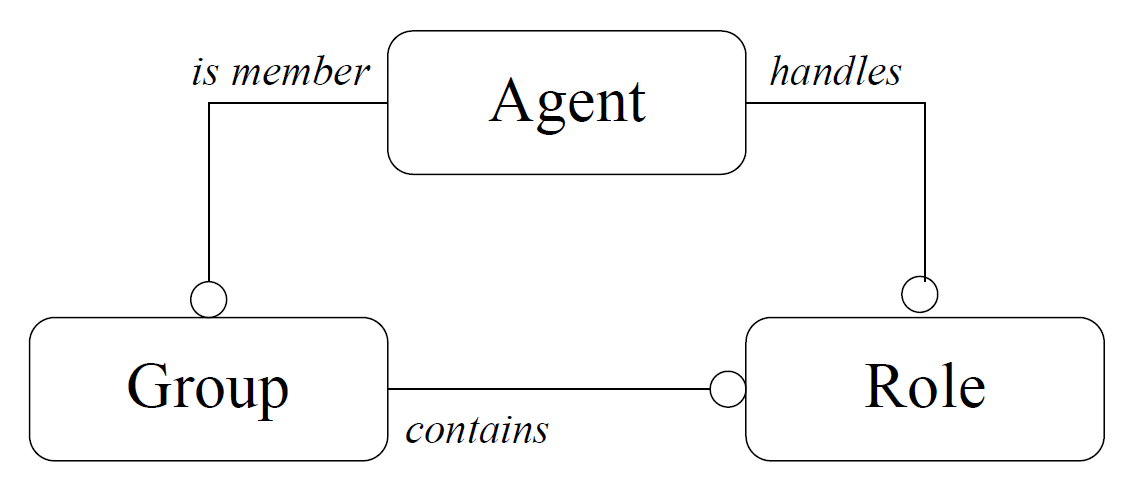
\includegraphics[width=0.5\textwidth]{images/aalaadin/core-model.png}
	\caption{The Aalaadin core model \cite{Ferber97}}
	\label{figure:aalaadin-core-model}
\end{figure}

\subsubsection*{Agent}

% Agent - definition
An \textit{agent} is defined in \cite{Ferber97} as an active communicating entity which plays \textit{roles} within \textit{groups}.

% Agent - no agent architecture imposed
Aalaadin does not prescribe any particular agent architecture.
Indeed, any metamodel striving for generality should impose as few constraints upon the resulting MAS models as possible.
After all, the decision of which agent architecture to employ is best made by the the MAS designer and relates to the MAS as such, not just its organizational structure.
As we will see, none of the metamodels introduced in this thesis force the MAS designer to adapt a concrete definition of agenthood.

\subsubsection*{Group}

% Group - definition
In \cite{Ferber97}, \textit{groups} are defined as atomic sets of agent aggregation.
% Group - about
In its most basic form, a group is just a way to tag a set of agents, it has no structure.
The real advantage of grouping agents becomes apparent when we introduce some structure to these groups.
This structure can be imposed using roles.

% Group - characteristics
Groups have the following characteristics:
\begin{itemize}
	\item An agent can be a member of a number of groups simultaneously.
	This means that group can overlap, which is major point of Aalaadin.
	\item A new group can be founded by any agent; an agent must request its admission to an existing group.
	\item A group may be local or distributed across multiple machines.
\end{itemize}

\subsubsection*{Role}

% Role - definition
A \textit{role} is an abstract representation of an agent function, service or identification within a group \cite{Ferber97}.
An agent can play multiple roles each of which is local to a group.
Similarly to group admission, playing a group in a role must be requested by the candidate agent (already belonging to the group) and awarded by the group founder agent.

% Role & communication
In Aalaadin, the communication is related to roles. Since an agent can play multiple roles, it can be engage in several independent dialogues simultaneously.

% Role - definition characteristics
The following characteristics are part of a role definition:
\begin{itemize}
	\item Uniqueness --  A role can be \textit{unique} or \textit{multiple} within a group.
	A unique role can be played by at most one agent in a group; a multiple role, on the other hand, can be played by any number of agents within a group. 
	\item Competences -- A \textit{competence} specifies a condition the candidate agent must satisfy to be eligible to play the role within the group. 
	\item Capacities -- A \textit{capacity} specifies an ability attributed to an agent while it is playing the role.
\end{itemize}
By default a role is multiple, does not require any competences and does not provide any capacities.

% Group manager role
A special role in a group is the \textit{group manager} role, which is automatically granted to the group founder.
It has a competence to handle group membership and role playing requests.
It also has a capacity to revoke roles and cancel group membership.

%%%%%%%%%%%%%%%%%%%%%%%%%%%%%%%%%%%%%%%%%%%%%%%%%%%%%%%%%%%%%%%%%%%%%%%%%%%%%%%%
\subsection{Methodological Concepts}

% Methodological model - about
The Aalaadin methodological model contains so-called \textit{methodological concepts}.
These concepts are not present directly in concrete organizations but only serve during the analysis and design phases.
Their purpose is to describe abstract organizations from which concrete organizations, described using the core concepts, will ultimately be derived.
Figure~\ref{figure:aalaadin-metamodel} illustrates the entire Aalaadin metamodel. The dotted ellipsis is the demarcation line between the core and methodological models.

% Figure: Aalaadin metamodel
\begin{figure}[h]
	\centering
	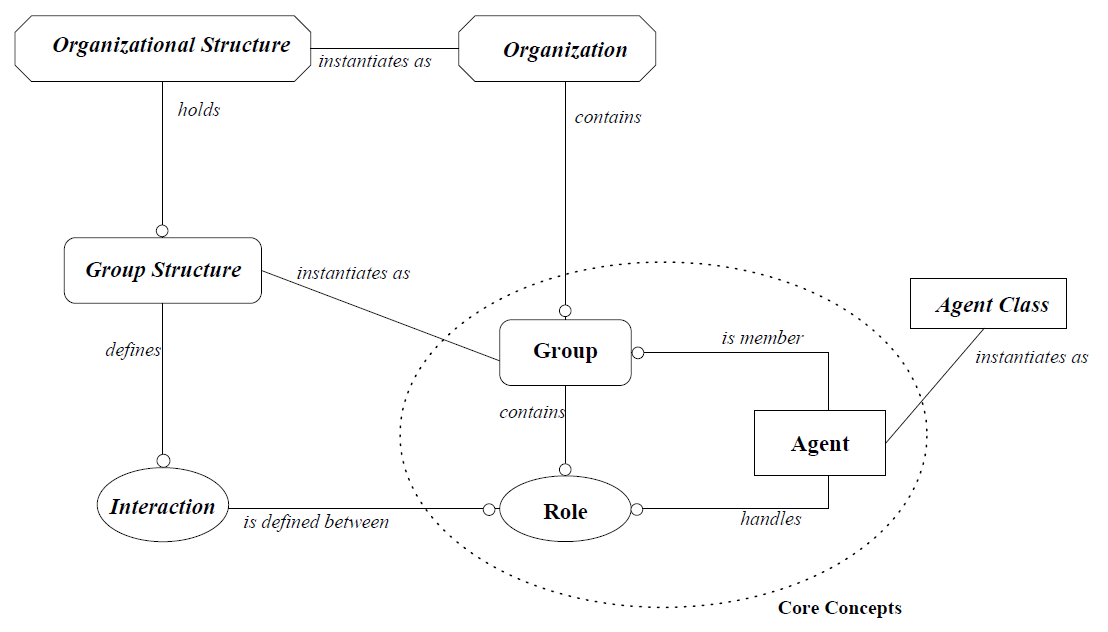
\includegraphics[width=0.75\textwidth]{images/aalaadin/aalaadin-metamodel.png}
	\caption{The Aalaadin metamodel \cite{Ferber97}}
	\label{figure:aalaadin-metamodel}
\end{figure}

\subsubsection*{Group Structure}

% Group structure - definition
A \textit{group structure} is an abstract description of a group \cite{Ferber97}.
It identifies all roles comprising the group and defines interactions among them.

% Group structure - definition characteristics
A group structure is defined by:
\begin{itemize}
	\item a list of available roles (see role definition) that can be played by agents in the group and
	\item a set of valid interaction schemes (including language) between roles.
\end{itemize}

% Group structure - partial instantiation
Note that an actual group might be a partial instantiation of its defining group structure.
This means that during the MAS execution, there might be a moment when some roles defined in the group structure are not played in a group.
This dynamic nature of groups allows for a great deal of run-time flexibility.

\subsubsection*{Organizational Structure}

% Organizational structure - definition
The \textit{organizational structure}, as defined in \cite{Ferber97}, is a set of group structures expressing the design of a multiagent organization scheme.

% Organizational structure - about
The organizational structure can be seen as the specification of the problem to be solved (organization to be modelled) using a MAS.
Any sort of heterogeneity within a single system (e.g. agent architecture or language heterogeneity) can be managed by different group structures involved in the organizational structure.

% Organizational structure - partial instantiation
Similarly to groups, an actual organization can be a incomplete manifestation of its defining organizational structure.
This means that while a MAS is being executed, there may be a point when some groups defined in the organizational structure are not present in an organization.
This also contributes to the overall run-time flexibility.

%%%%%%%%%%%%%%%%%%%%%%%%%%%%%%%%%%%%%%%%%%%%%%%%%%%%%%%%%%%%%%%%%%%%%%%%%%%%%%%%
\subsection{MadKit}

% MadKit - authors & references
The authors of Aalaadin also developed an agent platform implementing their metamodel called MadKit (Multi-Agent Development Kit)
\cite{Ferber97}, \cite{Ferber98} and \cite{Gutknecht00}.

% MadKit - basic philosophy
The basic philosophy of the Aalaadin/MadKit architecture is to use the platform itself for its own management wherever possible.
MadKit's main design principles are micro-kernel architecture and agentification of services;
all services except for the most fundamental ones provided by the micro-kernel are implemented as agents, organized in groups and identified by roles \cite{Ferber98}.